\documentclass[18pt]{beamer}

\usetheme{Madrid} % [secheader]
\setbeamertemplate{footline}{}
\usefonttheme{professionalfonts}
\usepackage[english]{babel}
\usepackage{graphicx}
\usepackage[normalem]{ulem}
\usepackage{hyperref}
\usepackage{bm}
\usepackage{dsfont}
\usepackage{subcaption}
\usepackage{bbm}
\usepackage{calc}  % For widthof command
\usepackage{xcolor}
\usepackage{tikz}
\usepackage{csquotes} % Necessary for biblatex.
\usepackage[
	style=authoryear-comp, 
	maxcitenames=2,
	natbib=true, 
	backend=bibtex
	]{biblatex}
\renewbibmacro{in:}{} % Remove "in" before the journal title.
\renewbibmacro{volume+number+eid}{} % Get rid of the volume and number.
\DeclareFieldFormat*{journaltitle}{\textit{#1}.}
\DeclareFieldFormat*{pages}{}
\DeclareFieldFormat*{urldate}{}
\newcommand{\fullauthorcite}[1]{
	\AtNextCite{\defcounter{maxnames}{99}}
	\fullcite{#1}
}
\addbibresource{hmc_lecture.bib}


\setbeamerfont{itemize/enumerate subbody}{size=\normalsize} %to set the body size
%\setbeamertemplate{frametitle}[default][center]
\setbeamertemplate{itemize subitem}{\normalsize\raise1.25pt\hbox{\donotcoloroutermaths$\blacktriangleright$}}  %to set the symbol size

% HMC related macros
\newcommand{\position}{\theta}
\newcommand{\momentum}{p}
\newcommand{\bposition}{\bm{\position}}
\newcommand{\bmomentum}{\bm{\momentum}}
\newcommand{\Position}{\Theta}
\newcommand{\Momentum}{P}
\newcommand{\Mass}{\bm{M}}
\newcommand{\integrationTime}{\tau}
\newcommand{\nIntegrationStep}{L}
\newcommand{\stepsize}{\Delta t}
\newcommand{\acceptprob}{a}
\newcommand{\solutionOp}{\bm{\Psi}}
\newcommand{\involution}{\bm{R}}

% Math macros
\newcommand{\transpose}{\text{\raisebox{.5ex}{$\intercal$}}}
\newcommand{\diff}{{\rm d}}
\newcommand{\Diff}{\mathbf{D}}
\DeclareMathOperator*{\argmax}{argmax}
\DeclareMathOperator*{\argmin}{argmin}

% Probability / statistics macros
\newcommand{\eqDistribution}{\mathrel{\raisebox{-.2ex}{$\overset{\scalebox{.6}{$\, d$}}{=}$}}}
\newcommand{\given}{\, | \,}
\newcommand{\normal}{\mathcal{N}}
\newcommand{\proposalKernel}{Q}
\newcommand{\indep}{\protect\mathpalette{\protect\independenT}{\perp}}
\def\independenT#1#2{\mathrel{\rlap{$#1#2$}\mkern2mu{#1#2}}}

% Variable / Greek symbol macros
\newcommand{\y}{\bm{y}}
\newcommand{\x}{\bm{x}}
\newcommand{\I}{\bm{I}}
\newcommand{\bPhi}{\bm{\Phi}}
\newcommand{\bSigma}{\bm{\Sigma}}
\newcommand{\nparam}{d}
\newcommand{\lshrink}{\lambda}
\newcommand{\gshrink}{\tau}

% Utility macros
\newcommand{\todo}[1]{\textcolor{red}{#1}}

% Fun macros
\newcommand{\shrug}[1][]{
	\begin{tikzpicture}[baseline, x=0.8\ht\strutbox, y=0.8\ht\strutbox, line width=0.125ex, #1]
	\def\arm{(-2.5,0.95) to (-2,0.95) (-1.9,1) to (-1.5,0) (-1.35,0) to (-0.8,0)};
	\draw \arm;
	\draw[xscale=-1] \arm;
	\def\headpart{(0.6,0) arc[start angle=-40, end angle=40,x radius=0.6,y radius=0.8]};
	\draw \headpart;
	\draw[xscale=-1] \headpart;
	\def\eye{(-0.075,0.15) .. controls (0.02,0) .. (0.075,-0.15)};
	\draw[shift={(-0.3,0.8)}] \eye;
	\draw[shift={(0,0.85)}] \eye;
	% draw mouth
	\draw (-0.1,0.2) to [out=15,in=-100] (0.4,0.95); 
	\end{tikzpicture}
}

% Custom environments
\newcommand{\defineWithinItemizeSpacing}{
	\setlength{\abovedisplayskip}{.3\baselineskip}
	\setlength{\belowdisplayskip}{.3\baselineskip}
}
\newenvironment{itemizedEquation}{
	\defineWithinItemizeSpacing
	\begin{equation}
}{
	\end{equation} \ignorespacesafterend
}
\makeatletter
\newenvironment{itemizedEquation*}{
	\defineWithinItemizeSpacing
	\begin{equation*}
}{
	\end{equation*} \ignorespacesafterend
}
\makeatother
\newenvironment{indented}{
	\hfill \begin{minipage}{\dimexpr\textwidth-3ex} 
}{
	\end{minipage}
}


% Color definitions
\definecolor{uclablue}{RGB}{39, 116, 174}
\definecolor{navyblue}{rgb}{0.0, 0.0, 0.5}
\definecolor{turquoise}{rgb}{0.19, 0.84, 0.78}
\definecolor{mediumturquoise}{rgb}{0.28, 0.82, 0.8}
\definecolor{lava}{rgb}{0.81, 0.06, 0.13}
\colorlet{linkColor}{mediumturquoise}
\colorlet{highlightedTextColor}{lava}


% Set the color theme of the presentation
\usecolortheme[named=uclablue]{structure}
\colorlet{textcolor}{white}
\setbeamercolor{frametitle}{fg=textcolor}
\setbeamercolor{titlelike}{fg=textcolor}
\setbeamercolor{section in head/foot}{fg=textcolor}
%\colorlet{toccolor}{black}
%\setbeamercolor{section in toc}{fg=toccolor}

\setbeamercolor{bibliography entry author}{fg=black}
\setbeamercolor{bibliography entry title}{use=structure, fg=structure.fg}
\setbeamercolor{bibliography entry note}{fg=black}

%  Block colors
\setbeamercolor{block title}{use=structure, fg=textcolor, bg=structure.fg}
\setbeamercolor{block body}{
	parent=normal text, use=block title, bg=block title.bg!10}
%\setbeamercolor{block title}{bg=uclablue!100, fg=white}


\setbeamertemplate{enumerate items}[default]
\setbeamerfont*{itemize/enumerate body}{size=\normalsize}
\setbeamerfont*{itemize/enumerate subbody}{parent=itemize/enumerate body}
\setbeamerfont*{itemize/enumerate subsubbody}{parent=itemize/enumerate body}

\setbeamercovered{dynamic}
\setbeamercovered{invisible}
\beamertemplatenavigationsymbolsempty

% Insert table of content frames between sections automatically. See http://en.wikibooks.org/wiki/LaTeX/Presentations
\AtBeginSubsection[]
{
  \begin{frame}
    \frametitle{Table of Contents}
    \tableofcontents[
    	  currentsection,
    	  sectionstyle=show/show,
    	  subsectionstyle=show/shaded/hide
    ]
	\end{frame}
}

\title[HMC: theory \& practice]{Hamiltonian Monte Carlo: Theory and Practice}
\author{Aki Nishimura\inst{1}}
\institute[]{Department of Biomathematics, University of California - Los Angeles \inst{1}}
\date{\today}


\begin{document}
\frame{\titlepage}


\section{Introducing Hamiltonian Monte Carlo (HMC)}


\subsection{Why \& What to learn about HMC}

\frame{
	\frametitle{What is HMC?}
	\begin{itemize}
	\item HMC is a state-of-the-art \textit{general-purpose} sampler, only requiring evaluation of the target log-density and its gradient.
	\item Required computations can be done algorithmically and efficiently for probabilistic models (or, more precisely, Bayesian networks):
		\begin{itemize}
		\item density evaluation via \textit{computational (directed acyclic) graphs} 
		\item gradient via \textit{reverse mode differentiation} / \textit{back-propagation}
		\end{itemize}
	\begin{figure}
		\centering
		\hspace{-.1\linewidth}
		
\includegraphics[height=.45\textheight]{Figure/probabilistic_programming_languages}
	\end{figure}
	\end{itemize}
}

\frame{
	\frametitle{What is HMC? (and what it is \textbf{not})}
	\begin{itemize}
	\item HMC is \textbf{not} a silver-bullet, though often good enough for computing posteriors of not-overly-complicated models with moderate sized data.
	\item HMC can be almost guaranteed to fail on certain target distributions.
		\begin{itemize}
		\item Work-arounds may exists in some cases, but not always.
		\end{itemize}
	\item Performance of HMC is sensitive to
		\begin{itemize}
		\item parametrization of the model.
		\item tuning parameters (which may be adjusted during a ``warm-up'').
		\end{itemize}
	\item In general, prefer
		\vspace{-.75\baselineskip}
		\begin{multline*}
		\text{model-specific inference algorithm by an expert} \\
			> \text{probabilistic programming implemnetation} \\
			> \text{your own code} \hspace{.05\linewidth}
		\end{multline*} \vspace{-1.5\baselineskip}
	\item When no other solid solutions exists, use Bayesian modeling and posterior computation via HMC as ``the least of all possible evils.''
	\end{itemize}
}

\frame{
	\frametitle{What is HMC? (and what it is \textbf{not})}
	\begin{itemize}
	\item Some softwares (e.g.\ \texttt{rstanarm}) incorporate model-specific best practices in applying HMC, yielding quite impressive performance.
	\item Some cutting-edge Bayesian methods rely on HMC for posterior computation with competitive computational efficiency.
		\begin{itemize}
		\item e.g.\ Bayesian sparse regression for GLM and survival analysis
		\end{itemize}
	\end{itemize}
}

\frame{
	\frametitle{Learning objectives: things to take home with}
	\begin{itemize}
	\item Sensitivity of HMC's performance means that, even as an end-user, one benefits from basic understandings of the algorithm.
	\item Hopefully, you will 
		\begin{itemize}
		\item know how to parametrize your model for best HMC performance.
		\item develop intuitions as to when posterior computation is feasible.
		\item be able to diagnose (and fix if possible) when sampling fails.
		\item know when to change default parameters in software packages.
		\item be familiar with research frontiers and improvements on the way.
		\end{itemize}
	\end{itemize}
}


\subsection{History \& Motivation behind HMC}

\frame{
	\frametitle{History of ``H''MC}
	\begin{itemize}
	\item Invented as ``hybrid'' Monte Carlo in computational physics literature for computer simulation of lattice models in quantum field theory.
	\item At the time, there were two dominant approaches:
		\begin{itemize}
		\item Monte Carlo simulation based on ``local'' moves, changing the state of one particle at a time.
		\item molecular dynamics simulation with ``global'' moves by numerically solving \textit{equations of motion}.
		\end{itemize}
	\item ``Hybrid'' Monte Carlo combined the efficiency of molecular dynamics with Metropolis algorithm to ensure the exact stationary distribution.
	\end{itemize}
}

\frame{
	\frametitle{What does Hamiltonian dynamics have to do with MCMC?}
	\begin{itemize}
	\item Two (often competing) objectives in constructing a proposal density:
		\begin{itemize}
		\item you want to make ``large" moves to explore the space. 
		\item you want sufficiently high acceptance rates.
		\end{itemize}
	\item e.g.\ random-walk Metropolis for $\nparam$-dimensional Gaussians:
		\begin{itemize}
		\item As $d \to \infty$, proposal variance needs to scale proportional to $1 / d$ to maintain a positive acceptance rate.
		\item With proposal variance $\propto 1 / d$, it takes $\nparam$ steps for the chain to travel a unit distance.
		\item Cost of generating one effective sample then is proportional to
			\begin{itemizedEquation*}
			\nparam \times \text{(cost of likelihood evaluation)}. 
			\end{itemizedEquation*}
		% Note: the cost is often described as $O(d^2)$ in the literature under the assumption that the likelihood evaluation costs $O(d)$.
		\end{itemize}
	\item Question: can we generate proposals that are far away from the current state, yet still maintains high acceptance rate? 
		\begin{itemize}
		\item Yes, use Hamiltonian dynamics to generate proposals! 
		\item In particular, HMC has the cost of $O(d^{1 / 4})$ in the above example.
		\end{itemize}
	\end{itemize}
}


\subsection{First look at HMC algorithm}

\frame{
	\frametitle{Set-up and terminologies for HMC}	
	\begin{itemize}
		\item To sample from the distribution of interest $\pi_\Position(\bposition)$, HMC augments the parameter space with an auxiliary parameter $\bmomentum \in \mathbb{R}^\nparam \sim \normal(\mathbf{0}, m \I)$.
		\item HMC then samples from the joint density
		\begin{itemizedEquation*}
		\pi(\bposition, \bmomentum) 
			\propto \pi_\Position(\bposition) \times \mathcal{N}\left( \bmomentum \, ; \mathbf{0}, m \I \right) 
		\end{itemizedEquation*}
		where $\bposition$ and $\bmomentum$ are referred to as \textit{position} and \textit{momentum} variables.
		\item HMC terminologies:
		\begin{itemize}
			\item $U(\bposition) = - \log \pi_\Theta(\bposition)$ : \textit{potential energy}.
			\item $K(\bmomentum) = \frac{1}{m} \bmomentum^\transpose \bmomentum$ : \textit{kinetic energy}.
			\item $H(\bposition, \bmomentum) = U(\bposition) + K(\bmomentum) = - \log \pi(\bposition, \bmomentum)$ : \newline \phantom{$H(\bposition, \bmomentum) = U(\bposition) + K(\bmomentum)$ =} \textit{Hamiltonian} or \textit{total energy}.
		\end{itemize}
	\end{itemize}
}

\frame{
	\frametitle{Transition kernel of HMC}
	\begin{itemize}
	\item HMC generates a proposal by combining momentum randomization and \textit{deterministic} transition of simulated Hamiltonian dynamics.
	\end{itemize}
	\begin{block}{HMC transition rule}
		Given the current state $(\bposition_0, \bmomentum_0)$, HMC generates the next state as follows:
		\begin{enumerate}
			\item Randomize momentum: $\bmomentum_0 \sim \mathcal{N}\left(\mathbf{0}, m \I \right)$.
			\item Generate a proposal $(\bposition^*, \bmomentum^*) \approx (\bposition(\integrationTime), - \bmomentum(\integrationTime))$ by approximating \newline the solution $\left\{ (\bposition(t), \bmomentum(t)) : t \in [0, \integrationTime] \right\}$ of \textit{Hamilton's equation}
				\vspace{-.3\baselineskip}
				\begin{equation} \label{eq:hamilton}
				\vspace{-.3\baselineskip}
				\begin{aligned}
				\frac{\diff \bposition}{\diff t} 
				&= m^{-1} \bmomentum, \quad
				\frac{\diff \bmomentum}{\diff t} 
				= - \nabla_{\bposition} U(\bposition) 
				\end{aligned}
				\end{equation}
				with initial condition $(\bposition(0), \bmomentum(0)) = (\bposition_0, \bmomentum_0)$.
			\item Accept or reject the proposal. 
				% with the probability $$ \min\left\{1, \pi(\bposition^*, \bmomentum^*) / \pi(\bposition, \bmomentum) \right\} $$
		\end{enumerate}
	\end{block}
}

\frame{
	\frametitle{Physical interpretation of HMC trajectories}
	\begin{itemize}
	\item Hamilton's equation describes a motion of a particle with mass $m$ under the potential energy field $U(\bposition)$:
		\begin{itemizedEquation*}
		\begin{aligned}
		\text{``velocity''}
			&= \frac{\diff \bposition}{\diff t} 
			= m^{-1} \bmomentum
			\\
		\text{``mass $\times$ acceleration''}
			&= \frac{\diff \bmomentum}{\diff t} 
			= - \nabla_{\bposition} U(\bposition) 
			= \text{``force''}
		\end{aligned}
		\end{itemizedEquation*}
	\item Trajectory $\bposition(t)$ accelerates toward lower values of the potential $U(\bposition)$ or, equivalently, larger values of $\log \pi_\Position(\bposition) = - U(\bposition)$.
	\end{itemize}
}

\frame{
	\frametitle{Visual illustration: HMC in action}
	\begin{center}
	\href{run:Figure/hmc_in_action_2d_Gaussian.avi}{\color{linkColor} \fontsize{16pt}{18pt} \selectfont HMC for a 2d Gaussian (correlation $= 0.9$)}
	\vspace{4ex}

	\href{run:Figure/hmc_in_action_2d_Gaussian_slow_motion.avi}{\color{linkColor} \fontsize{16pt}{18pt} \selectfont Click here for slow motion version}
	\end{center}
}


\section{Theory of HMC: exactness \& high acceptance rate}

\subsection{Exactness of HMC at stationarity}

\frame{
	\frametitle{HMC as a valid Metropolis algorithm}
	\begin{itemize}
	\item Hamiltonian dynamics generates a \textit{symmetric} proposal 
	\begin{itemizedEquation*}
	\proposalKernel\left\{ (\bposition, \bmomentum) \to (\bposition^*, \bmomentum^*)  \right\}
		= \proposalKernel\left\{ (\bposition^*, \bmomentum^*) \to (\bposition, \bmomentum) \right\}
	\end{itemizedEquation*}
	by virtue of its \textit{reversibility} (and \textit{volume-preservation}).
		\begin{itemize}
		\item For a deterministic proposal kernel, interpret the symmetry as
		\begin{itemizedEquation*}
		\proposalKernel\left\{ S \to S^* \right\}
			= \proposalKernel\left\{ S^* \to S \right\}
		\end{itemizedEquation*}
		for a pair of sets $S$ and $S^*$.
		\end{itemize}
	\item Evolution of Hamiltonian dynamics can be ``reversed'' (or ``inverted'') by flipping momentum and applying the same dynamics:
		\begin{itemizedEquation*}
		(\bposition, \bmomentum) \to (\bposition', \bmomentum')
			\quad \Leftrightarrow \quad
			(\bposition', -\bmomentum') \to (\bposition, -\bmomentum)
		\end{itemizedEquation*}
	\end{itemize}
}

\frame{
	\frametitle{Symmetry via reversibility of Hamiltonian dynamics}
	\begin{itemize}
	\item Let $\{ \solutionOp_t \}_{t \in \mathbb{R}}$ denote the \textit{solution operator} of dynamics i.e.\ 
		\begin{itemizedEquation*}
		(\bposition(t), \bmomentum(t)) := \solutionOp_t(\bposition, \bmomentum)
		\end{itemizedEquation*}
		solves Hamilton's equations and $\solutionOp_0(\bposition, \bmomentum) = (\bposition, \bmomentum)$.
	\item Let $\involution(\bposition, \bmomentum) = (\bposition, - \bmomentum)$ denote the momentum flip operator.	
	\item \textit{Reversibility} of dynamics means that
		\begin{itemizedEquation*}
		\left( \involution \circ \solutionOp_t \right)^{-1} = \involution \circ \solutionOp_t 
			\ \text{ for all } \ t \in \mathbb{R}.
		\end{itemizedEquation*}
	\end{itemize}
	\vspace{-.5\baselineskip}
	\begin{figure}
	\centering
	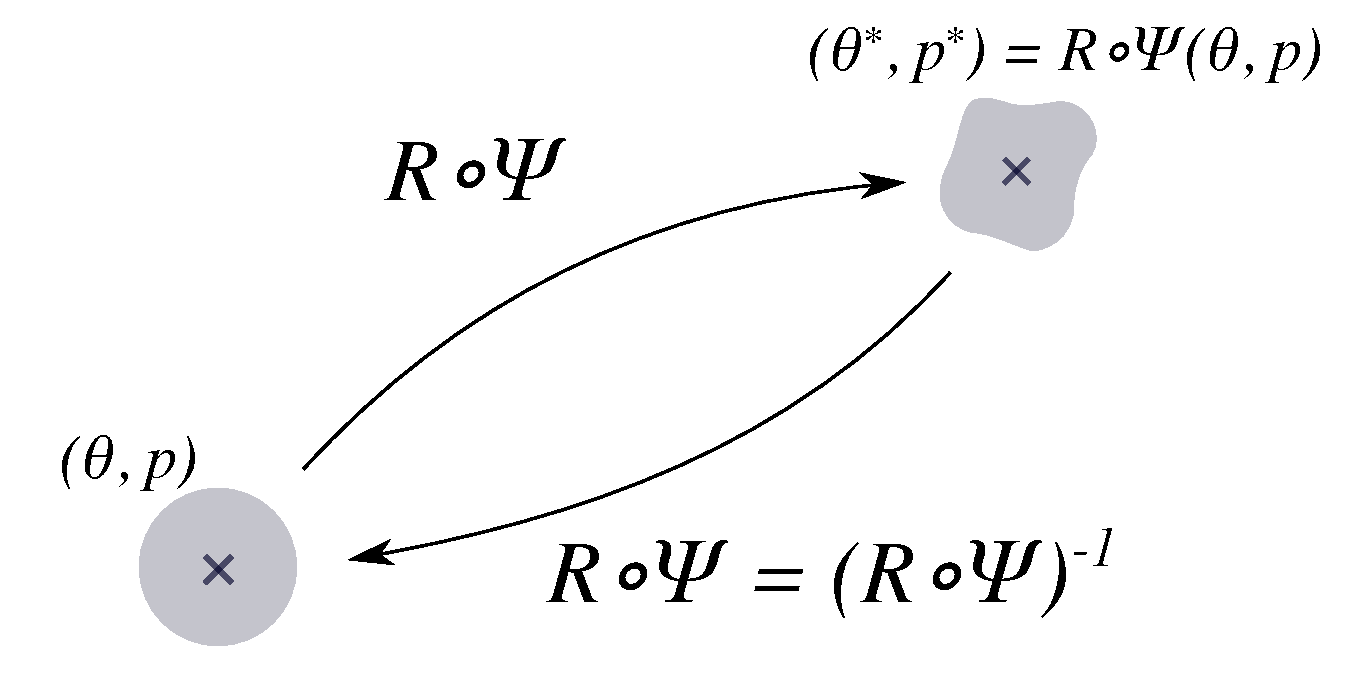
\includegraphics[height=.45\textheight]{Figure/reversible_map}
	\end{figure}
}

\frame{
	\frametitle{Geometric / structure-preserving numerical integration}
	\begin{itemize}
	\item In practice, Hamiltonian dynamics must be numerically approximated.
	\item \textit{Integrator} refers to an algorithm for approximating solutions of ODEs.
	\item For an approximate dynamics to remain a valid proposal mechanism, the integrator must preserve reversibility (and volume-preservation).
	\item To approximate the evolution from time $t$ to $t + \stepsize$ of dynamics
		\begin{itemizedEquation*}
		\frac{\diff \bposition}{\diff t} 
			= m^{-1} \bmomentum, \quad
		\frac{\diff \bmomentum}{\diff t} 
			= - \nabla U(\bposition),
		\end{itemizedEquation*}
		the \textit{leapfrog} (or \textit{velocity Verlet}) method carries out the updates
		\begin{itemizedEquation*}
		\arraycolsep=2pt
		\def\arraystretch{1.75}
		\begin{array}{ccccc}
		\bmomentum_{t + \stepsize / 2}
			&=& \bmomentum_t 
			&-& \displaystyle \frac{\stepsize}{2} \nabla U(\bposition_t) \\
		\bposition_{t + \stepsize}
			&=& \bposition_t
			&+& \stepsize \, m^{-1} \bmomentum_{t + \stepsize / 2} \\
		\bmomentum_{t + \stepsize}
			&=& \bmomentum_{t + \stepsize / 2}
			&-& \displaystyle \frac{\stepsize}{2} \nabla U(\bposition_{t + \stepsize}).
		\end{array}
		\end{itemizedEquation*}
	\item Map $\solutionOp_{\stepsize}^\nIntegrationStep$ induced by $\nIntegrationStep(\tau) = \lfloor \tau / \stepsize \rfloor$ steps of the leapfrog updates approximate the exact evolution from time $t = 0$ to $t = \integrationTime$. 
	\end{itemize}
}

\subsection{High acceptance rate of HMC proposals}

\frame{
	\frametitle{Invariance of the target under Hamiltonian dynamics}
	\begin{itemize}
	\item If we could solve Hamiltonian dynamics exactly, then HMC proposals would have $100\%$ (!) acceptance rates.
	\item In essence, this is because the target $\pi(\cdot, \cdot)$ is an \textit{invariant} distribution of the dynamics --- if $(\bposition, \bmomentum) \sim \pi(\cdot, \cdot)$, then $\solutionOp_t(\bposition, \bmomentum) \sim \pi(\cdot, \cdot)$ for all $t$.
	\item With numerical approximation, acceptance rate of HMC proposals  converges to 1 as $\stepsize \to 0$ for a fixed $\tau$ and $\nIntegrationStep(\tau) = \lfloor \tau / \stepsize \rfloor$.
		% TODO : later provide a more quantitative discussion of the error as a function of stepsize.
	\end{itemize}
}

\frame{
	\frametitle{Acceptance probability of reversible map proposals}
	\begin{itemize}
	\item For a general reversible map $\solutionOp$, the correct acceptance probability of a proposal $(\bposition^*, \bmomentum^*) = \solutionOp(\bposition, \bmomentum)$ is given by 
		\begin{itemizedEquation*}
		\min \! \left\{
			1, \, \frac{
				\pi(\bposition^*, \bmomentum^*) \left| \Diff \solutionOp(\bposition, \bmomentum) \right|
			}{
				\pi(\bposition, \bmomentum)}
		\right\}
		\end{itemizedEquation*}
		\vspace{-.5\baselineskip}
		\begin{itemize}
		\item To see why the Jacobian is needed, recall that the density of a transformed variables $(\bposition^*, \bmomentum^*) = \solutionOp(\bposition, \bmomentum)$ is given as
			\begin{itemizedEquation*}
			\pi_{\Position^*, \, \Momentum^*}(\bposition^*, \bmomentum^*) 
				= \pi_{\Position, \, \Momentum}(\bposition, \bmomentum) \left| \Diff \solutionOp(\bposition, \bmomentum) \right|^{-1}.
			\end{itemizedEquation*}
		\end{itemize}
	\item Hamiltonian dynamics and its leapfrog approximation are both volume-preserving, meaning $\left| \Diff \solutionOp_{\integrationTime} \right| = \left| \Diff \solutionOp_{\stepsize}^\nIntegrationStep \right| = 1$.
	\item Hence, the acceptance probability of an HMC proposal is
		\begin{itemizedEquation*}
		\min \! \left\{
			1, \, \frac{
				\pi(\bposition^*, \bmomentum^*)
			}{
				\pi(\bposition, \bmomentum)}
		\right\}
			= \min \! \left\{
				1, \, \exp\!\big( H(\bposition, \bmomentum) - H(\bposition^*, \bmomentum^*) \big)
			\right\}.
		\end{itemizedEquation*}
	\end{itemize}
}

\frame{
	\frametitle{Energy-conservation property for high acceptance rate}
	\begin{itemize}
	\item Hamiltonian dynamics is \textit{energy-conserving}, meaning the Hamiltonian remains constant along its trajectory $(\bposition(t), \bmomentum(t))$:
		\begin{itemizedEquation*}
		H(\bposition(t), \bmomentum(t)) 
			= H(\bposition(0), \bmomentum(0))
			\ \text{ for all } \ t.
		\end{itemizedEquation*}
	\item With the leapfrog approximation for a fixed $\integrationTime$,  the error is
		\begin{itemizedEquation*}
		\Delta H
			= H(\bposition_{\nIntegrationStep \stepsize}, \bmomentum_{\nIntegrationStep \stepsize})
				- H(\bposition_{0}, \bmomentum_{0})
			= O(\stepsize^2).
		\end{itemizedEquation*}
	\item Metropolis proposals in general satisfies, as $\Delta H \to 0$,
		\begin{itemizedEquation*}
		\mathbb{E}\left[ \Delta H \right]
			\approx \frac{1}{2} \, \mathbb{E}\left[ \Delta H^2 \right]
		\end{itemizedEquation*}
		% Note: we have an actual bound $E[\Delta H] \leq E[\Delta H^2]$ for a reversible dynamics-based proposal.
		% Note: the above relation holds for any Metropolis type algorithm
	\item HMC proposals thus satisfies $\mathbb{E}[\Delta H] = O(\stepsize^{\textcolor{highlightedTextColor}{4}})$ as $\stepsize \to 0$.
	\item e.g.\ HMC generates one effective sample from $\nparam$-dimensional Gaussians with the cost of
		\begin{itemizedEquation*}
		\nparam^{1 / 4} \times \text{(cost of likelihood \& gradient evaluation)}.
		\end{itemizedEquation*}
	\end{itemize}
}

\subsection{Summary \& 2nd look at HMC algorithm}

\frame{
	\frametitle{Summary: theory of HMC}
	\begin{itemize}
	\baselineskip=16pt
	\item Reversibility (\& volume-preservation) of Hamiltonian dynamics \\
		\hspace*{2em} $\Rightarrow$ Symmetry of HMC proposals \\
		\hspace*{5em} $\Rightarrow$ HMC as a valid Metropolis algorithm
		\vspace{.5\baselineskip}
	\item Volume-preservation \& Energy-conservation \\
		\hspace*{2em} $\Rightarrow$ Invariance of the target under Hamiltonian dynamics \\
		\hspace*{5em} $\Rightarrow$ High acceptance rate of HMC proposals
	\end{itemize}
}

\frame{
	\frametitle{Another look at HMC transition kernel}
	\vspace{-.3\baselineskip}
	\begin{itemize}
	\item Having covered details, we now state the algorithm more precisely.
		\begin{itemize}
		\item \textit{Mass} $\Mass = \textrm{Var}(\bmomentum)$ need not to be proportional to the identity.
		\item Momentum flip is optional since $\pi(\bposition, \bmomentum) = \pi(\bposition, -\bmomentum)$.
		\end{itemize}
	\end{itemize}
	\vspace{-.3\baselineskip}
	\begin{block}{HMC transition rule}
		Given the current state $(\bposition_0, \bmomentum_0)$, HMC generates the next state as follows:
		\begin{enumerate}
			\item Randomize momentum: $\bmomentum_0 \sim \mathcal{N}\left(\mathbf{0}, \textcolor{highlightedTextColor}{\Mass} \right)$.
			\item Generate a proposal $(\bposition^*, \bmomentum^*) \approx (\bposition(\integrationTime), \textcolor{highlightedTextColor}{\pm} \bmomentum(\integrationTime))$ \textcolor{highlightedTextColor}{by using the leapfrog integrator} to approximate the solution of Hamilton's equation
				\vspace{-.5\baselineskip}
				\begin{equation}
				\vspace{-.5\baselineskip}
				\begin{aligned}
				\frac{\diff \bposition}{\diff t} 
				&= \textcolor{highlightedTextColor}{\Mass^{-1}} \bmomentum, \quad
				\frac{\diff \bmomentum}{\diff t} 
				= - \nabla_{\bposition} U(\bposition) 
				\end{aligned}
				\end{equation}
				with initial condition $(\bposition(0), \bmomentum(0)) = (\bposition_0, \bmomentum_0)$.
			\item Accept or reject the proposal \textcolor{highlightedTextColor}{with the acceptance probability
				\begin{itemizedEquation*}
				\min\left\{1, \pi(\bposition^*, \bmomentum^*) / \pi(\bposition, \bmomentum) \right\}.
				\end{itemizedEquation*}
				} \vspace{-\baselineskip}
		\end{enumerate}
	\end{block}
}

\frame{
	\frametitle{Another look at HMC transition kernel}
	\vspace{-.3\baselineskip}
	\begin{itemize}
	\item Same theories justify a  more general version below.
		\begin{itemize}
		\item Any symmetric, potentially position-dependent, distribution can be employed for momentum: $- \bmomentum \given \bposition \eqDistribution \bmomentum \given \bposition \sim \pi_{\Momentum \given \Position}(\, \cdot \given \bposition)$.
		\item Note: a \textit{symplectic} integrator is reversible and volume-preserving.
		\end{itemize}
	\end{itemize}
	\vspace{-.3\baselineskip}
	\begin{block}{HMC transition rule}
		Given the current state $(\bposition_0, \bmomentum_0)$, HMC generates the next state as follows:
		\begin{enumerate}
			\item Randomize momentum: \textcolor{highlightedTextColor}{$\bmomentum_0 \given \bposition_0 \sim \pi_{\Momentum \given \Position}(\, \cdot \given \bposition_0)$}.
			\item Generate a proposal $(\bposition^*, \bmomentum^*) \approx (\bposition(\integrationTime),  \bmomentum(\integrationTime))$ by using \textcolor{highlightedTextColor}{a reversible and volume-preserving integrator} to solve Hamilton's equation
				\vspace{-.5\baselineskip}
				\begin{equation}
				\vspace{-.5\baselineskip}
				\begin{aligned}
				\frac{\diff \bposition}{\diff t} 
				&= \textcolor{highlightedTextColor}{\nabla_{\bmomentum} K(\bposition, \bmomentum)}, \quad
				\frac{\diff \bmomentum}{\diff t} 
				= - \nabla_{\bposition} U(\bposition) 
				\end{aligned}
				\end{equation}
				with initial condition $(\bposition(0), \bmomentum(0)) = (\bposition_0, \bmomentum_0)$.
			\item Accept or reject the proposal with the acceptance probability
				\begin{itemizedEquation*}
				\min\left\{1, \pi(\bposition^*, \bmomentum^*) / \pi(\bposition, \bmomentum) \right\}.
				\end{itemizedEquation*}
				 \vspace{-\baselineskip}
		\end{enumerate}
	\end{block}
}


\section{Case study: HMC on Gaussian targets}

\frame{
	\frametitle{Table of Contents}
	\tableofcontents[
		currentsection,
		sectionstyle=show/shaded,
		subsectionstyle=show/shaded/hide
	]
}

\frame{
	\frametitle{HMC on univariate Gaussian target}
	\begin{itemize}
	\item We first consider HMC's behavior for $\position \sim \normal(0, \sigma^2)$, $\momentum \sim \normal(0, 1)$ or
		\begin{itemizedEquation*}
		U(\position) =  \frac{\position^2}{2 \sigma^2}, \ \
		K(\momentum) =  \frac{\momentum^2}{2}.
		\end{itemizedEquation*}
	\item Corresponding dynamics is described by
		\begin{itemizedEquation*}
		\frac{\diff \position}{\diff t} = \momentum, \ \
		\frac{\diff \momentum}{\diff t} = - \frac{\position}{\sigma^2}
			\ \ \text{ or equivalently } \ \
			\frac{\diff^2 \position}{\diff t^2} = - \frac{\position}{\sigma^2}
			.
		\end{itemizedEquation*}
	\item Solution coincides a harmonic oscillator with period $2 \pi \sigma$:
		\begin{itemizedEquation*}
		\position(t) 
			= \position_0 \cos(t / \sigma) + \momentum_0 \, \sigma \sin(t / \sigma).
			% , \ \ \momentum(t) = \dot{\position}(t)
		\end{itemizedEquation*}
	\item If $\position_0 \sim \normal(0, \sigma^2)$ and $\momentum_0 \sim \normal(0, 1)$, then $\position(t) \sim \normal(0, \sigma^2)$ for all $t$ and \vspace{-.7\baselineskip}
		\begin{itemizedEquation*}
		\position(\integrationTime) 
			= \momentum_0 \, \sigma 
			\indep \position_0
			\ \text{ for } \ \integrationTime = \pi \sigma / 2.
		\end{itemizedEquation*}
	\end{itemize}
}

\frame{
	\frametitle{Leapfrog dynamics \& stability limit on integrator stepsize}
	\begin{itemize}
	\item In case of a Gaussian target, one leapfrog can be expressed as
		\begin{itemizedEquation*}
		\begin{bmatrix}
		\bposition_{n \stepsize} \\ \bmomentum_{n \stepsize}
		\end{bmatrix}
			= 
			{\def\arraystretch{1.5}
			\begin{bmatrix}
			1 - \frac{\stepsize^2}{2 \sigma^2} & \stepsize \\
			- \frac{\stepsize}{\sigma^2} + \frac{\stepsize^3}{4 \sigma^4} & 1 - \frac{\stepsize^2}{2 \sigma^2}
			\end{bmatrix}
			}
			\begin{bmatrix}
			\bposition_{(n - 1) \stepsize} \\ \bmomentum_{(n - 1) \stepsize}
			\end{bmatrix}.
		\end{itemizedEquation*}
	\item Eigenvalues of the leapfrog map $\solutionOp_{\stepsize}$ have magnitude $< 1$ if and only if the stepsize is within the \textit{stability region} $\stepsize < 2 \sigma$.
	\item For $\stepsize > 2 \sigma$, the acceptance rate effectively drops to 0.
	\end{itemize}
}

\frame{
	\frametitle{Leapfrog dynamics \& stability limit on integrator stepsize}
	\begin{itemize}
	\item For $\stepsize < 2 \sigma$, we have the following formula for $\solutionOp_{\stepsize}^n$:
		\begin{itemizedEquation*}
		\begin{bmatrix}
		\bposition_{n \stepsize} \\ \bmomentum_{n \stepsize}
		\end{bmatrix}
			= 
			\arraycolsep=0pt
			\begin{bmatrix}
			\cos(n \phi) 
				& \sigma \left( 1 - \frac{\stepsize^2}{4 \sigma^2} \right)^{\text{\tiny $-1/2$}} \sin(n \phi) \\
			- \frac{1}{\sigma} \left( 1 - \frac{\stepsize^2}{4 \sigma^2} \right)^{\text{\tiny $1/2$}} \sin(n \phi) 
				& \cos(n \phi)
			\end{bmatrix}	
			\begin{bmatrix}
			\bposition_{0} \\ \bmomentum_{0}
			\end{bmatrix}
		\end{itemizedEquation*}
		where $\phi = \phi(\stepsize / \sigma) = \cos^{-1}\!\left( 1 - \frac{\stepsize^2}{2 \sigma^2} \right)$.
	\item Since $\cos^{-1}(1 - \delta^2 / 2) \approx \delta$, we have $ n \phi \approx n \stepsize / \sigma$ as $\stepsize / \sigma \to 0$.
	\item For $\stepsize$ sufficiently small, a choice $\nIntegrationStep \approx \frac{\pi \sigma}{2 \stepsize}$ yields
		\begin{itemizedEquation*}
		\cos(L \phi) \approx 0
			\ \text{ \& } \sin(L \phi) \approx 1
		\end{itemizedEquation*}
	and the proposal $(\bposition_{\nIntegrationStep \stepsize},  \bmomentum_{\nIntegrationStep \stepsize})$ approximately independent of $(\bposition_{0},  \bmomentum_{0})$. 
	\end{itemize}
}

\frame{
	\frametitle{Acceptance rate  / Hamiltonian error as function of stepsize}
	\begin{itemize}
	\item Acceptance probability is given as $\min\{1, \exp(-\Delta H)\}$ where 
		\begin{itemizedEquation*}
		\Delta H 
			= - \log \frac{
					\pi(\bposition_{\nIntegrationStep \stepsize},  \bmomentum_{\nIntegrationStep \stepsize})
				}{
					\pi(\bposition_{0},  \bmomentum_{0})
				}.
		\end{itemizedEquation*}
	\item After tedious calculation, we can show that
		\begin{itemizedEquation*}
		\mathbb{E} \left[ \Delta H \right]
			= \frac{\stepsize^4}{\sigma^4} 
				\left( 1 - \frac{\stepsize^2}{4 \sigma^2} \right)^{-1}
				\frac{\sin^2(\nIntegrationStep \phi)}{32}.
		\end{itemizedEquation*}
	\end{itemize}
	\begin{figure}
	\centering
		\begin{minipage}{.5\linewidth}
		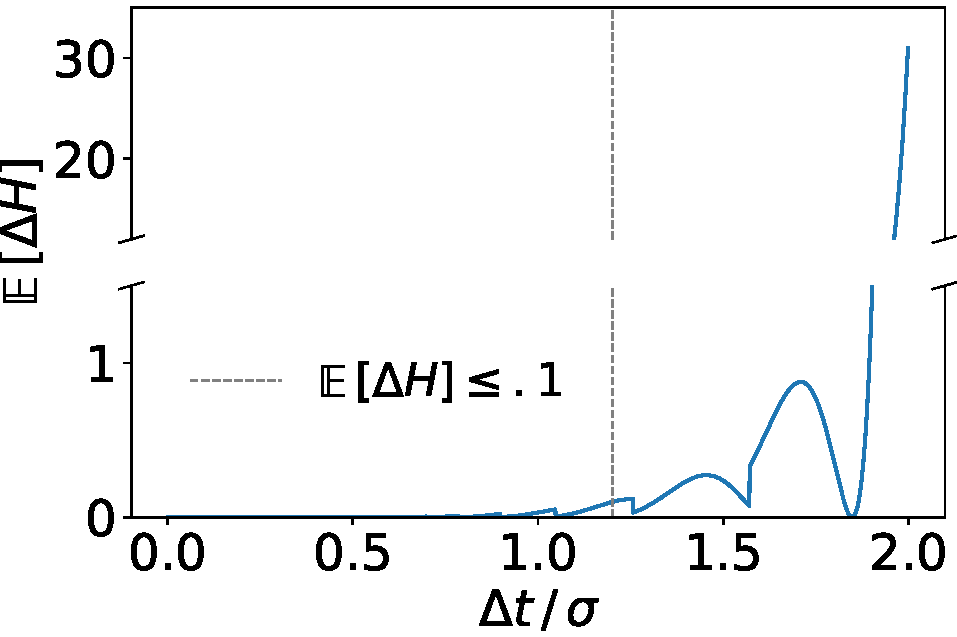
\includegraphics[height=.4\textheight]{Figure/ave_hamiltonian_error_on_gaussian_target}
		\end{minipage}
		\begin{minipage}{.425\linewidth}
		\vspace{-\baselineskip}
		\caption{Average Hamiltonian error $\mathbb{E} \left[ \Delta H \right]$ as a function of $\stepsize$ \\ when $\integrationTime = 2 \pi \sigma$ and $\nIntegrationStep = \lceil \integrationTime / \stepsize \rceil$.}
		\end{minipage}
	\end{figure}
}

\frame{
	\frametitle{HMC on multivariate Gaussians}
	\begin{itemize}
	\item Consider the target $\bposition \sim \normal(\bm{0}, \bm{\Sigma})$, $\bmomentum \sim \normal(\bm{0}, \I)$.
	\item With the identity mass, HMC's performance turns out to be invariant under rotation of the parameter i.e.\ we can assume that $\bSigma$ is diagonal.
	\item With $U(\bposition) = \sum_{i = 1}^\nparam \frac{\position_i}{2 \sigma_i^2}$ and $K(\bmomentum) = \sum_{i = 1}^\nparam \frac{p_i^2}{2}$, Hamilton's equation decouples into $\nparam$ independent one-dimensional equations:
		\begin{itemizedEquation*}
		\frac{\diff \position_i}{\diff t} = \momentum_i, \ \
		\frac{\diff \momentum_i}{\diff t} = - \frac{\position_i}{\sigma_i^2}
			\ \ \text{ for } \ \
			i = 1, \ldots, \nparam.
		\end{itemizedEquation*}
	\item Leapfrog update also decouples into one-dimensional updates:
		\begin{itemize}
		\item Direction with the \textit{smallest} variance determines the overall stability limit of $\stepsize < 2 \min_i \sigma_i$.
		\item Direction with the \textit{largest} variance determines the necessary number of leapfrog steps $L \approx \frac{\pi}{2 \stepsize} \max_i \sigma_i$.
		\item Error accumulates over the coordinates: $\Delta H = \sum_i \Delta H_i$.
		\end{itemize} 
	\end{itemize}
}

\frame{
	\frametitle{Computational cost of HMC on multivariate Guassians}
	\begin{itemize}
	\item Computational cost is $\propto L \propto \frac{\sigma_{\max}}{\stepsize}$. What $\stepsize$ to use?
	\item Stability limit is $\stepsize < 2 \sigma_{\min}$, but $\Delta H$ needs to be controlled too.
	\item In an extreme case $\sigma_i = \sigma_0$ for all $i$'s, we have
		\begin{itemizedEquation*}
		\mathbb{E}\left[ \Delta H \right]
			= \nparam \times \mathbb{E} \left[ \Delta H_1 \right]
			\propto \nparam \times \stepsize^4.
		\end{itemizedEquation*}
		\vspace{-\baselineskip}
		\begin{itemize}
		\item Need $\Delta t \propto d^{-1/4}$ to maintain a positive acceptance rate.
		\item Computational costs becomes $\propto \sigma_{\max} \, d^{1 / 4}$.
		\end{itemize}
	\item In another extreme case $\sigma_{\min} \ll \sigma_i$ for $i \neq \argmin_j \sigma_j$, the error is completely dominated by $\Delta H_{\argmin_i \sigma_i}$. 
		\begin{itemize}
		\item Since $\mathbb{E} \left[ \Delta H_i \right] \propto \stepsize / \sigma_i$ and $\stepsize < 2 \sigma_{\min}$, there are little contributions to the overall error from $\Delta H_i$ for $i \neq \argmin_j \sigma_j$. 
		\item Computational costs becomes $\propto \sigma_{\max} / \sigma_{\min}$ --- the ratio \\ between the largest and smallest ``widths'' of the target.
		\end{itemize}
	\end{itemize}
}



\section{Tuning HMC: theory and practice}

\frame{
    \frametitle{Table of Contents}
    \tableofcontents[
    	  currentsection,
    	  sectionstyle=show/shaded,
    	  subsectionstyle=show/shaded/hide
    ]
}

\frame{
	\frametitle{Tuning parameters of HMC}
	\begin{itemize}
	\item Performance of HMC depends critically on the choice of
		\begin{itemizedEquation*}
		\arraycolsep=2pt
		\def\arraystretch{1.2}
			\begin{array}{ccl}
			\Mass
				&:& \text{mass matrix} \\
			\integrationTime \, \text{ or } \, L = \lfloor \integrationTime / \stepsize \rfloor
				&:& \text{integration time\, or\, path length} \\
			\stepsize 
				&:& \text{integrator stepsize}
			\end{array}
		\end{itemizedEquation*}
	\item Bayesian software packages automatically tune these parameters behind the scene.
		\begin{itemize}
		\item These tuning algorithms yet again have tuning parameters (!). The default values are reasonable, but certainly not perfect.
		\item Manual adjustment of the tuning algorithm parameters is often necessary.
		\end{itemize}
	\end{itemize} 
}


\subsection{Mass matrix for preconditioning target distribution}

\frame{
	\frametitle{Mass matrix for linear parameter transformation}
	\begin{itemize}
	\item \textbf{Fact :} HMC's performance remains identical whether sampling from the (joint) parameter space $(\bm{A} \bposition, \bmomentum)$ and from $(\bposition, \bm{A}^\transpose \bmomentum)$.
	\item When using the identity mass $\Mass = \I$, 
		\begin{itemize}
		\item the computational cost tends to increase as the ratio between the largest and smallest ``widths'' of the target does.
		\item (linear) reparametrization $\bposition \to \bSigma^{-1/2} \bposition$ for $\bSigma = \text{Var}(\bposition)$ often improves the efficiency.
		\end{itemize}
	\item In other words, we expect HMC to perform best when sampling from the transformed parameter $\bSigma^{-1/2} \bposition$ with $\bmomentum \sim \normal(\bm{0}, \I)$.
	\item Equivalently, we can sample from the original parameter $\bposition$ but with a transformed momentum $\bSigma^{-1/2} \bmomentum \sim \normal(\bm{0}, \Mass = \bSigma^{-1})$.
	\item Summary: choose $\Mass = \text{Var}(\bposition)^{-1}$ to sample effectively from $\bSigma^{-1/2} \bposition$.
	\end{itemize}
}

\frame{
	\frametitle{Tuning mass matrix in practice}
	\begin{itemize}
	\item In real-life, reparametrization $\bSigma^{-1/2} \bposition$ may not be optimal e.g.\ a target can have the identity covariance with all sorts of complex geometries.
	\item When $\pi_\Position(\bposition)$ is log-concave, the Hessian of $- \log \pi_\Position(\bposition)$ is a locally optimal choice for the mass matrix.
		% Note: information theory backs up this statement to an extent, but to my knowledge this is not a proven statement.
	\item What about more general cases? Who knows \shrug.
	\item But let's say we aim for $\Mass = \text{Var}(\bposition)^{-1}$ as commonly done.
		\begin{itemize}
		\item $\bSigma$ can be estimated during the ``warm-up \!/\! burn-in'' period.
		\item Empirical covariance is unstable in high-dimensions; we may estimate the marginal variances only and set $\Mass = \textrm{diag}(\bm{\widehat{\Sigma}})^{-1}$.
		\item As the non-identity mass has an effect of implicit transformation $\bposition \to \Mass^{1/2} \bposition$, choice of $\Mass$ and of $\stepsize$ interact with each other.
		\item We want to keep the narrowest ``width'' of the distribution of $\Mass^{1/2} \bposition$ constant, so scale $\Mass$ to have the smallest eigenvalue $1$.
		\end{itemize}
	\end{itemize}
}

\subsection{Integration time --- decisive factor on HMC mixing rate}

\frame{
	\frametitle{Choosing integration time \\ {} \hfill \& Automating choice via No-U-turn criteria}
	\begin{itemize}
	\item Integration time $\integrationTime$ determines how ``far'' a proposal $(\bposition^*, \bmomentum^*) \approx (\bposition(\integrationTime), - \bmomentum(\integrationTime))$ is from the current state.
	\item For a Gaussian target, we saw the optimal integration time to be
		\begin{itemizedEquation*}
		\integrationTime \approx \frac{\pi}{2} \times \text{the target's widest ``width''}.
		\end{itemizedEquation*}
	\item ``$\integrationTime \propto \text{width}$'' is a useful way of thinking, but provides no practical guidance in general settings.
	\item One possibility is to empirically calibrate $\integrationTime$ to maximize a performance metric such as an \textit{expected jumping distance}.
	\item Reliable, generally efficient, and simpler alternative is to use the \textit{no-U-turn} algorithm to obviate the need for manually choosing $\integrationTime$.
	\end{itemize}
}

\frame{
	\frametitle{No-U-turn algorithm for automating integration time}
	\begin{itemize}
	\item No-U-turn algorithm is often described as a version of HMC, but can be used with any reversible dynamics-based samplers.
	\item No-U-turn sampler (NUTS) refers to HMC + No-U-turn algorithm.
	\item \textbf{Motivation}: Trajectories of Hamiltonian dynamics, if simulated long enough, typically start turning back toward where it started. 
		\begin{itemize}
		\item Recall the harmonic oscillation in the Gaussian case.
		\item More generally, $\frac{\diff \bmomentum}{\diff t} = - \nabla_{\bposition} U(\bposition)$ means that the velocity $\frac{\diff \bposition}{\diff t}$ will eventually point toward the mode of the target.
		\end{itemize}
	\item Simulating trajectories is likely wasteful beyond the \textit{U-turn} time
		\begin{itemizedEquation*}
		\begin{aligned}
		\integrationTime_{\textsc{u}}
			&= \min_{t > 0} \left\{
				\frac{\diff}{\diff t} \left\| \bposition(t) - \bposition_0 \right\|^2 < 0
			\right\} \\
			&= \min_{t > 0} \left\{
				\big\langle \bposition(t) - \bposition_0, \Mass^{-1} \bmomentum(t) \big\rangle < 0
			\right\}.
		\end{aligned}
		\end{itemizedEquation*}
	\item Map $(\bposition_0, \bmomentum_0) \to (\bposition(\integrationTime_{\textsc{u}}), - \bmomentum(\integrationTime_{\textsc{u}}))$ is \emph{not} reversible, but no-U-turn algorithm ensures the symmetry of proposals via recursive simulation of trajectories in forward and backward directions.
	\end{itemize}
}


\subsection{Integrator stepsize: accuracy \& computational cost trade-off}

\frame{
	\frametitle{Choosing integrator stepsize: accuracy \& cost trade-off}
	\begin{itemize}
	\item We need $\stepsize$ small enough to achieve a reasonable acceptance rate but smaller values require more gradient evaluations $L = \lfloor \integrationTime / \stepsize \rfloor$.
	\item Acceptance rate $\acceptprob(\stepsize)$ is a reasonable and easy-to-estimate metric for tuning $\stepsize$: $\acceptprob(\stepsize) \approx 0$ $\Leftrightarrow$ $\stepsize$ too large \& $\acceptprob(\stepsize) \approx 1$ $\Leftrightarrow$ $\stepsize$ too small.
	\item Once we specify a target acceptance rate, a stochastic optimization algorithm can be used to solve for the corresponding $\stepsize$. 
	\item What is a good target acceptance rate?
		\begin{itemize}
		\item \cite{beskos2013optimal-hmc} show $0.651$ to be optimal under high-dimensional i.i.d.\ distributions.
		\item \cite{betancourt2014hmc-stepsize} say $0.6 \sim 0.9$, with larger values more robust in practice.
		\item Stan's default is $0.8$.
		\item I say start with $0.9$ and further decrease $\stepsize$ when you notice frequent instability / divergence of simulated trajectories. \\
			(Also, in situations where $0.651$ is indeed optimal, using $0.9$ instead incurs only a modest additional cost, say $40\%$.)
		\end{itemize}
	\end{itemize}
}

\frame{
	\frametitle{Case for conservative (smaller) stepsizes}
	\begin{itemize}
	\item Why aim for $a(\stepsize) \geq 0.9$? \\
		--- because real-life posteriors are often much more complex than those for which theoretically optimal acceptance rates are derived.
	\item For a complex target distribution, a specified stepsize may appear to approximate dynamics accurately until the numerical approximation suddenly breaks down in some regions of the parameter space.
	\item This occurs when the stability limit of the integrator varies across the parameter space. See below for an example:
	\begin{figure}
		\begin{minipage}{.48\linewidth}
		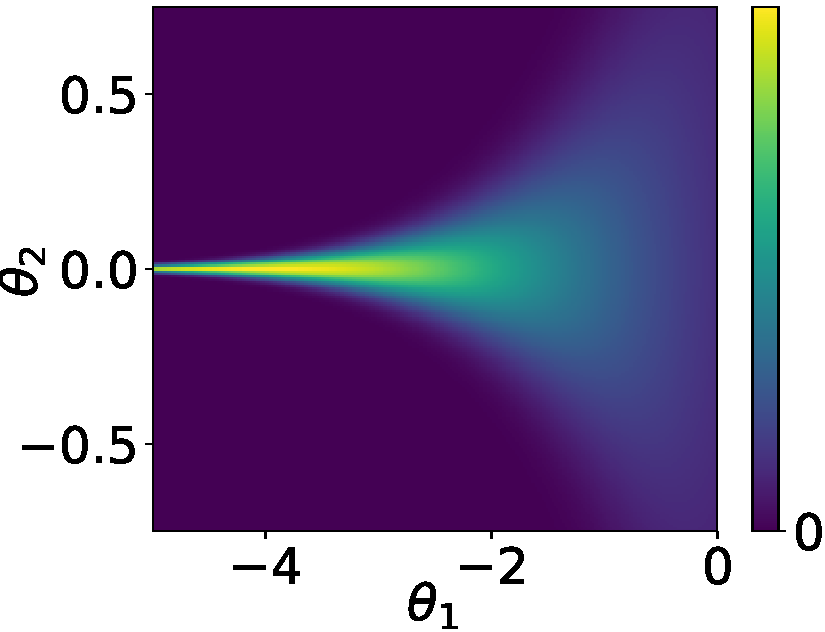
\includegraphics[height=.4\textheight]{Figure/2d_funnel_distribution}
		\end{minipage}
		\begin{minipage}{.48\linewidth}
		\caption{
			Density of the target \\ 
			\hspace*{2ex} $\position_2 \given \position_1 \sim \normal(0, \text{scale} =  \exp(\position_1))$ \\
			\hspace*{2ex} $\position_1 \sim \normal(0, \text{scale} = 2)$. \\
			The stability limit of the integrator is $\bposition$-dependent and is approximately $\exp(\position_1)$ when $\Mass = \I$.
			In this toy example, an obvious solution is to sample from $(\position_1, \position_2 / \exp(\position_1))$.
		}
		\end{minipage}
	\end{figure}
	\end{itemize}
}

\frame{
	\frametitle{Case for conservative (smaller) stepsizes}
	\begin{itemize}
	\item Another important point --- also related to the issue of stability limit --- is that HMC requires rather specific tail conditions.
		% Note: if using Gaussian momentum and the leapfrog integrator. 
	\item Example: $\pi_\Position(\position) \sim \exp(-|\position|^\alpha)$ as $\position \to \pm \infty$ 
		\begin{itemize}
		\item HMC is geometrically ergodic if and only if $1 \leq \alpha \leq 2$.
		\end{itemize}
	 \item Example: $\position \sim \textrm{Exp}(1) \geq 0$
	 	\begin{itemize}
	 	\item Sampling from $\position' = \log \position$ is a common practice to avoid having to deal with the constraint $\position \geq 0$. But for $\position \sim \textrm{Exp}(1)$ we  have
 		 	\begin{itemizedEquation*}
 		 	\pi_{\log \Position}(\position')
 		 		= \exp \left( \position' - e^{\position'} \right)
 		 	\end{itemizedEquation*}
		 and HMC on $\position'$ is provably \emph{not} geometrically ergodic!
	 	\end{itemize}
	\end{itemize}
}

\frame{
	\frametitle{Practically, if not provably, small enough stepsize for HMC}
	\begin{itemize}
	\item Um, it sounds like HMC does \emph{not} work on many target distributions? \\
		--- Yes, but don't worry about it.
		\hspace*{-1ex} ...\ I mean, avoid obvious problems but otherwise proceed and later check for potential issues.
	\item In practice, we are typically concerned with regions of highest density, not where ``$\| \bposition \| \to \infty$.''
	\item Stability limit on $\stepsize$, if restricted to a high density region, is almost surely bounded below.
	\end{itemize}
}

\frame{
	\frametitle{Practically, if not provably, small enough stepsize for HMC}
	\begin{itemize}
	\item In other words, $\stepsize$ just need to be small enough for the integrator to remain stable within a high density region.
	\item I know, it may not sound like an ideal solution, but theory almost never coincides with practice: get over with it.
		\begin{itemize}
		\item Target distributions, if potentially problematic to HMC, are likely problematic to other algorithms as well.
			% Note: though HMC may be a bit more sensitive.
		\end{itemize}
	\item Reparametrization can solve, or at least alleviate, some problems.
	\item Alternative choice of momentum distributions leads to HMC variants more robust to the numerical stability issues.
	\end{itemize}
}

\subsection{Summary}

\frame{
	\frametitle{Summary / Guide on tuning HMC}
	\begin{itemize}
	\item Mass matrix $\Mass$:
		\begin{itemize}
		\item Modifying $\Mass$ coincides with linearly transforming the target.
		\item Common choices are $\Mass = \widehat{\bSigma}^{-1}$ or $\Mass = \textrm{diag}(\widehat{\bSigma})^{-1}$. 
		\end{itemize}
	\item Integration time $\integrationTime$:
		\begin{itemize}
		\item Should be proportional to the ``width'' of the target.
		\item No-U-turn algorithm provides a generally good solution.
		\end{itemize}
	\item Integrator stepsize $\stepsize$:
		\begin{itemize}
		\item In complex models, the stability condition often limits its size.
		\item Set a high target acceptance rate (e.g.\ $0.9$) for peace of mind.
		\item When instability persists for very small $\stepsize$, it's time to look into reparametrization or even alternative models.
		\end{itemize}
	\end{itemize}
}


\section{Deploying HMC in practice: best practices and useful techniques}

\frame{
    \frametitle{Table of Contents}
    \tableofcontents[
    	  currentsection,
    	  sectionstyle=show/shaded,
    	  subsectionstyle=show/shaded/hide
    ]
}

\frame{
	\frametitle{Automated tuning of HMC / NUTS}
	\begin{itemize}
	\item Let's look at how Stan (\& other softwares) tune the HMC parameters.
	\item Stan uses ``warm-up'' iterations to adapt the integrator stepsize and mass matrix. (Terminology: \texttt{warm-up = burn-in + tuning}.)
	\begin{figure}
	\centering
	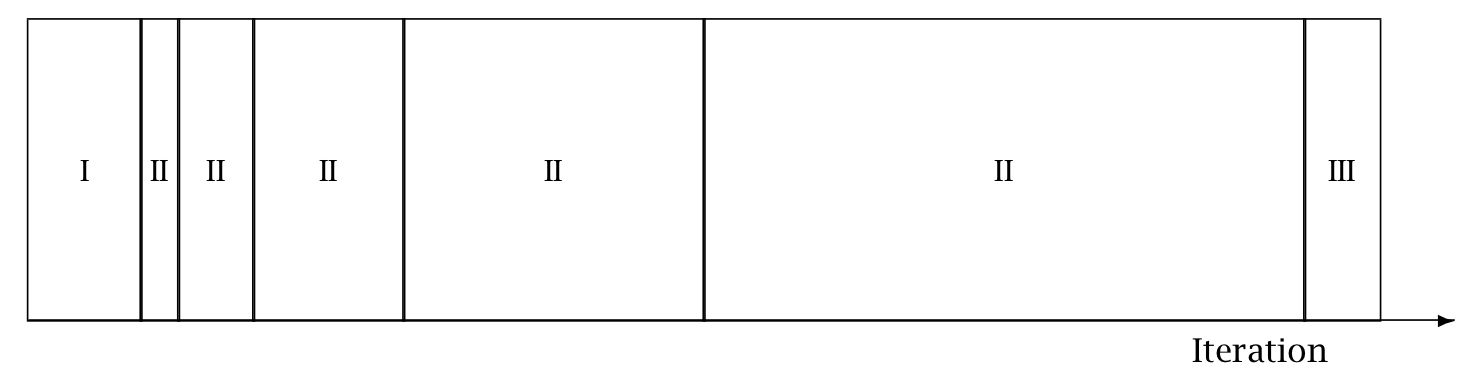
\includegraphics[width=\linewidth]{Figure/stan_adaptation_visuallization}
	\end{figure}
	\item Adaptation occurs in three stages: 1) stepsize only, 2) both stepsize \& mass matrix over multiple windows, 3) stepsize only.
	\item Lengths of adaptation are controlled by parameters \texttt{adapt\_init\_buffer}, \texttt{adapt\_term\_buffer}, and \texttt{adapt\_window}.
	\end{itemize}
}

\frame{
	\frametitle{Handling constrained and discrete parameters}
	\begin{itemize}
	\item Parameters often take values in a constrained space e.g.\ variances, correlation matrices, number of species, etc.
	\item Hamiltonian dynamics underlying HMC does not natively support constrained or discrete spaces.
	\item For constrained parameters, the standard approach is to map them to unconstrained ones. For example,
		\begin{itemize}
		\item $\sigma > 0$ : $\sigma \to \log \sigma$
		\item $q \in [0, 1]$ : $q \to \log(q / (1 - q))$
		\item $\text{correlation matrix} \to \text{partial correlations}$.
		\end{itemize}
	\item For discrete parameters, some options exist but no established one:
		\begin{itemize}
		\item Stan do not support them (at least as of April, 2019).
		\item PyMC updates them conditionally on the continuous parameters.
		\item Discontinuous HMC of \citet{nishimura2017discontinuous-hmc} extends HMC to accommodate ordinal discrete parameters. Adopted by \citet{gram2018dhmc-for-probabilistic-programs}, but not yet widely available.
		\end{itemize}
	\end{itemize}
}

\frame{
	\frametitle{Initializing Markov chain with reasonable values}
	\begin{itemize}
	\item Thoughtless initialization (e.g.\ through Stan default) often yields a state \emph{nowhere near} the stationarity.
	\item Shape of the target distribution near the initial state and at stationarity --- and hence appropriate stepsize and mass matrix --- may be totally different!
	\item Poor initialization can thus delay HMC to reach stationarity and to find a reasonable stepsize and mass matrix. 
	\item Good ways to initialize?
		\begin{itemize}
		\item Sampling an initial state from a prior, when using an informative one, is probably better than the software default.
		\item Run an optimization algorithm to find a local mode of the target. (PyMC takes a step further and uses a variational inference.)
		\end{itemize}
	\end{itemize}
}

\frame{
	\frametitle{Re-parametrizing to decouple model parameters}
	\begin{itemize}
	\item Alternative parametrizations of equivalent models can make substantial differences in computational tractability of the posteriors.
	\item In the Gaussian example, we saw the computational cost of HMC (when $\Mass = \I$) to increase as the correlations increase.
		\begin{itemize}
		\item Diagonal mass matrix can account for differences in scale among the coordinates, but not the correlation structure.
		\end{itemize}
	\item More generally, if we can reduce dependence among the parameters, posterior computation becomes easier.
	\item Example: parameters $(\beta, \sigma)$ with structure $\beta \given \sigma \sim \normal(0, \sigma^2)$ and $\sigma \sim \pi_{\Sigma}(\cdot)$ can be re-parametrized as $(\tilde{\beta} = \beta / \sigma , \sigma)$ so that $\tilde{\beta} \indep \sigma$.
	\end{itemize}
}

\frame{
	\frametitle{Scaling model parameters to comparable units}
	\begin{itemize}
	\item Magnitude of posterior uncertainty tend to be proportional to the scale of a parameter.
	\item e.g.\ if regressing ``income (usd)'' and ``years in school'' on some outcome, the income coefficient will likely have a smaller variance.
	\item Diagonal mass can account for the scale differences, but empirical adaptation may take significantly longer if the parameters are on vastly different scales to begin with.
	\item If the parameters are obviously on different scales, therefore, you might as well rescale them before fitting the model.
	\end{itemize}
}

\subsection*{References}

\frame{
	\frametitle{References}
	\begin{indented}
	Many wisdoms in addressing practical issues can be found in 
	\end{indented}
		\begin{itemize}
		\item \fullauthorcite{stan18}
		\end{itemize}
	\begin{indented}
	Details on Stan's tuning algorithm can be found at 
	\end{indented}
		\begin{itemize}
		\item \fullauthorcite{stan-hmc-params}
		\end{itemize}
	\begin{indented}
	Common types of problematic posteriors (and ways to deal with or avoid them) are described at
	\end{indented}	
		\begin{itemize}
		\item \fullauthorcite{stan-problematic-posterior}
		\end{itemize}
	\begin{indented}
	R package \texttt{rstanarm} provides wrapper functions of models written in optimized Stan codes:
	\end{indented}
		\begin{itemize}
		\item \fullauthorcite{rstanarm}
		\end{itemize}
}


\end{document}